\documentclass[11pt, letterpaper]{article}

  \title{\LaTeX\ for Linguistics}
  \author{Nicholas LaCara \\ University of Toronto}
  \date{Draft -- April 2019}
  
    %% Document-internal hyperlinks
    \usepackage[breaklinks, colorlinks, linkcolor=blue]{hyperref}
  
    %% The geometry package manipulates page margins
    \usepackage{geometry}
    
    %% Different fonts.
%     \usepackage[T1]{fontenc}
% 	\usepackage[bitstream-charter]{mathdesign}
% 	\usepackage{newpxtext,eulerpx}

    %% For denotation brackets
    \usepackage{stmaryrd}
      
    %% For LaTeX logos
    \usepackage{metalogo}
    
    %% For phonetic symbols and characters
    \usepackage{tipa}
    
    %% For in-document url formatting
    \usepackage{url}
    
    %% For drawing arrows
    \usepackage{pst-node}
    
    \usepackage{pst-asr}
    
    %% For drawing trees
    \usepackage{pst-jtree}
    
    %% For drawing trees with bracket notation
    \usepackage{tikz}
    \usepackage{tikz-qtree}
    
    \usepackage[linguistics]{forest}
    
    %% For nice OT Tableaux
    \usepackage[open, medium, round]{OTtablx}
    
    %% For sequentially numbered examples
    \usepackage{gb4e}
    
    
  %% This is an example command I introduce later in the document.
  \newcommand{\highlight}[1]{\underline{\textbf{#1}}}

\begin{document}
  
  \maketitle
  
  \tableofcontents
  
  \newpage
%   \section{Introduction}
  
  \section{Background}
  
    \begin{itemize}
      \item \LaTeX\ (pronounced \textipa{["lA.tEx]} or \textipa{["lA.tEk]}, \textipa{["leI.tEk]}\ldots) is a popular system for typesetting technical documents in the fields of math, physics, engineering, and linguistics.
      
      \item It has native support for typesetting complex mathematical formulas:
      
	$$ i \hbar \frac{\partial}{\partial t}\vert\Psi(\mathbf{r},t)\rangle = \hat H\vert\Psi(\mathbf{r},t)\rangle $$
	
	\item Many of \LaTeX's features are useful for linguists and all academic and technical writers:
	
	  \begin{itemize}	    
	    \item Built-in sectioning and reference commands allow for easy structuring of documents and intra-document cross-references.
	    
	    \item The inbuilt math support is used for technical notation in all subfields.

	    \item The bibliography system (Bib\TeX) allows for easy citation management and outputs formatted reference sections.	    

	  \end{itemize}

      
      \item It has been expanded in various ways over the years to accommodate Linguistics, as well:
      
	  \begin{itemize}
	    
	    \item Extensions (known as packages) for drawing trees, tableaux, and other linguistic representations have been developed which allow for creating consistent, professional-looking diagrams and graphics.
	    
	    \item Other extensions allow for simple input of \textsc{ipa} characters
	  \end{itemize}
      
% 	\begin
    \end{itemize}
    
  
  \subsection{Why use \LaTeX?}
  
    \LaTeX\ is known to have a fairly steep learning curve, especially for those who are not used to coding or programming, though I think part of this reputation is undeserved.
    
      \begin{itemize}
	\item Unlike what-you-see-is-what-you-get word processors (\textsc{wysiwyg}; Microsoft Word, LibreOffice Write, and Google Docs), \LaTeX\ makes it difficult to format your documents in an arbitrary way.
	
	\item Things that are easy to do in Word are often hard to do in \LaTeX. Think of this as a good thing: Part of the philosophy of using \LaTeX is maintaining consistent formatting throughout a document. This means that some formatting options are intentionally difficult to change on a whim.
	
	\item Many users coming from a \textsc{wysiwyg} background are not used to having so much control taken away from them. But the idea is that an author should concentrate less on the formatting and more on the content and structure of the document they are composing.
	
      \end{itemize}

    \noindent \LaTeX\ has a number of technical features that 
  
      \begin{itemize}
	
	\item Built-in support for technical document structures and cross-referencing.
	
	\item Macros and custom commands allow for easy and consistent formatting throughout a document.
		
	\item Many linguistics-specific packages for typesetting and referencing examples, drawing trees, creating Optimality Theory tableaux
	
	\item Lack of formatting options, in principle, allows for focus on document structure.
	
      \end{itemize}
      
    \noindent Furthermore, it is free software (no cost, no commercial limitations).
    
      \begin{itemize}
	\item In principle, this means that it will be available in perpetuity for free.
	\item .tex files can be opened with any text editor on any computer.
        \item \LaTeX\ code will produce the same output no matter what system it is compiled on.
      \end{itemize}


  \subsection{What it's not}
  
    \begin{itemize}
%       \item \LaTeX\ is a scripting language that instructs an interpretor on how to format documents.

      \item \LaTeX\ is not a word processor, and you really shouldn't use it like one.
      
% 	  \begin{itemize}
      
	    \item I once co-edited a \textsc{nels} proceedings, and I edited a paper where the author had encoded section titles with commands like \verb|\noindent\textbf{1. Introduction}| rather than using the built-in \verb|\section| command that would have done this formatting for them.
	    
	    \item This is what is meant when people say that \LaTeX\ allows the author to focus on the content and structure rather than formatting. The sectioning commands (see Section \ref{S:Structure}) ensure the same consistent formatting is always used while building a structure for the document.
      
% 	  \end{itemize}
      
    \end{itemize}

  \subsection{This document}
  
    \begin{itemize}
      \item The goal of this document is to provide novice and inexperienced users with a guide for using \LaTeX\ to create and typeset linguistics documents, though it is probably also of use to those outside of linguistics.
      
      \item The source code for this document has, as a result, been kept relatively simple and straightforward to make it easy to compare with the compiled document; only the minimal number of packages necessary have been used to create this document.
    \end{itemize}


  \section{Getting it}
  
  \subsection{MacOS}
  
    \begin{itemize}
      \item There are a couple of different ways of installing \LaTeX\ on MacOS.
      
      \item A simple way is to use the Mac\TeX\ distribution.
      
      \item Alternatively, one can use MacPorts to install \TeX live.
    \end{itemize}


  \subsection{Windows}
  
    \begin{itemize}
	\item Windows users can download and install MiK\TeX.
    \end{itemize}

  \subsection{Linux}
  
    \begin{itemize}
	\item Most popular \textsc{gnu}/Linux distributions (Ubuntu, Fedora, Linux Mint\ldots) include \LaTeX\ in their repositories. The following commands will install the full \LaTeX\ distribution (around 4ish \textsc{gb}):
	
	  \begin{itemize}
	  
	    \item Ubuntu: \verb|$ sudo apt-get install texlive-full|
	    \item Fedora: \verb|# yum install texlive-scheme-full|
	  
	  \end{itemize}
	  
    \end{itemize}
      
  \subsection{The internet}\label{S:Internet}
  
    \begin{itemize}
      \item If you aren't ready to take the plunge, if you can't get the Mik\TeX\ installer to work, or if you just want to play around, there are websites that allow you to use \LaTeX\ online.
      
      \item Overleaf (\url{https://www.overleaf.com/}) allows for collaborative online editing of documents.
    \end{itemize}

      
  \section{Workflow}
  
  \subsection{Compiling a document}\label{S:Compiling}
  
    \begin{itemize}
    
	\item One of the main ways that using \LaTeX\ differs from using a word processor is the need to \emph{compile} a document. That is, it is necessary to convert the \LaTeX\ code into a human-readable .pdf file.
    
      \item There are different ways to compile a document, using different compilers. The compiler you need to use might depend on the packages you choose; most full \LaTeX\ installations will install all three following ones.
      
	  \begin{itemize}
	  
	    \item I raise this now since it raises compatibility issues for some packages that are useful for linguistics. 
	    
	    \item I'll point these compatibility issues out when they are relevant.
	  
	  \end{itemize}
      
      \item The “traditional” way is to send your document to the \LaTeX compiler. This creates a .dvi file that must be converted to a .ps file and then to a .pdf file.
      
	\begin{verbatim}
	  $ latex document.tex
	  $ dvips document.dvi
	  $ ps2pdf document.ps
	\end{verbatim}
	
	\item The script \verb|latexmk| automates this process (see more below).
	

      \item However, pdf\LaTeX\ will produce a .pdf file directly. The resulting .pdf file is generally cleaner than th
      
	\begin{verbatim}
	  $ pdflatex document.tex
	\end{verbatim}
	
      \item Another option is \XeLaTeX, which will produce a .pdf directly, as well. \XeLaTeX\ provides several additional extensions to \LaTeX, including native \textsc{utf8} support and the ability to use all the fonts installed on your computer.
      
	\begin{verbatim}
	  $ xelatex document.tex
	\end{verbatim}
	

      \item Because of how the system interacts with external databases for things such as citations and document-internal references, you may need to compile the document more than once.
      
%       \item 
%       
    \end{itemize}
    
  \subsection{Compiling with Bib\TeX\ and other}
  
    \begin{itemize}
      \item One of the chief advantages to using \LaTeX\ is that it automates compiling bibliographies from in-line citations. This is usually done with a bibliography management system known as Bib\TeX\ (see Section \ref{S:Bib}).
      
      \item Because of the way this works, you will have to compile your document several times.
      
	  \begin{itemize}
	  
	    \item The first compilation identifies the citations in your document and creates a list of these citations to search for in a bibliography file (this list is stored in a .aux file).
	    
	    \item Running Bib\TeX\ will take the list of citations and search for them in the bibliography file, creating the references section for the document you are creating (which is stored in a .bbl file).
	    
	    \item Compiling the document a second time will integrate the contents of the .bbl file with your original document.
	    
	    \item Compiling the document a third time will link the in-line citations to the references that have been added to your document.
	  
	  \end{itemize}
	  
	\item This means that if you are using plain \LaTeX, you will have to use the following commands to produce a .pdf file if you change the citations in the document:
	
	\begin{verbatim}
	  $ latex document.tex
	  $ bibtex document.aux
	  $ latex document.tex
	  $ latex document.tex
	  $ dvips document.dvi
	  $ ps2pdf document.ps
	\end{verbatim}
	
	\item As noted above, the script \verb|latexmk| automates this process, detecting changes to your .aux and .bbl files and running commands as necessary.
	
	\item Using a \LaTeX-specific editor can also automate this process.

    \end{itemize}


  \subsection{Using a \LaTeX-specific editor}
  
    \begin{itemize}
      \item There are many text editors designed specifically around composing \LaTeX\ documents. While many hardcore coders seem to gravitate toward other editors, I think using a \LaTeX-specific editor is good for beginners as they  often provide a \textsc{gui} that simplifies the many of the repetitive processes that go into creating and compiling a document.
      
      \item The editors available depend on your system.
      
	  \begin{itemize}
	  
	    \item TeXshop on MacOS is very popular.
	    
	    \item Kile is a very versatile editor available on Linux.
	  
	  \end{itemize}
      
      \item Additionally, Overleaf, mentioned in Section \ref{S:Internet}, also provides a web interface for compiling documents.
    \end{itemize}

      
  \section{Basics of a \LaTeX\ document}
  
    \begin{itemize}
      \item A \LaTeX\ document is just a plain text document containing \LaTeX\ code.
      
      \item That code is processed by an interpreter that creates a formatted document from that plain text code.
    \end{itemize}

  
  \subsection{Preamble}
  
  \subsubsection{Document class}
  
    \begin{itemize}
      \item The document class tells \LaTeX\ what kind of document you are creating. This can affect various commands made available to you.
      
      \item The document class must be declared at the beginning of your document with the \verb|documentclass| command.
      
	\begin{exe}
	  \ex \verb!\documentclass[<options>]{<class>}! 
	\end{exe}

      
      \item For our purposes, the \verb|article| class will be sufficient, and the instructions in this document will be assume you are using \verb|article|, but there are several other classes available, including \verb|report|, \verb|book|, \verb|memoir|, and \verb|letter|.
      
      \item The \verb|article| class makes available a number of options, which can be separated by commas:
      
	\begin{exe}
	  \ex \begin{tabular}[t]{ll}
	        \textsc{Option}: 	& \textsc{Function}: \\
% 	      \hline
	        \verb|10pt| 		& Sets font size to 10pt \\
	        \verb|11pt| 		& Sets font size to 11pt \\
	        \verb|12pt| 		& Sets font size to 12pt \\
	        \verb|a4paper|		& Sets paper size to A4 \\
	        \verb|a5paper|		& Sets paper size to A5 \\
	        \verb|draft|		& Marks material that flows into the right margin \\
	        \verb|letterpaper| 	& Sets paper size to US Letter \\
	        \verb|titlepage|	& Causes \verb|\maketitle| to print title on separate page \\
		  \verb|twocolumn|	& Prints text in two columns (but use the package \verb|multicol| instead). \\
	        \verb|twoside|		& Sets different margins on even and odd pages \\
	      \end{tabular}

	\end{exe}

      \item To create an 11pt document on letter paper, start your document with the following command:
      
	\begin{exe}
	  \ex \verb!\documentclass[11pt, letterpaper]{article}! 
	\end{exe}

	
    \end{itemize}

  \subsubsection{Title, author, and date}
  
    \begin{itemize}
      \item You can declare the title of your document and the author with the \verb|\title| and \verb|\author| commands.
      
	  \begin{exe}
	    \ex \verb|\title{\LaTeX\ for Linguists}|
	    \ex \verb|\author{Nicholas LaCara}|
	  \end{exe}
	
      \item There are no specific commands for other identifying information, unfortunately. If you want to include information like your affiliation, as I've done in this document, you can include a line break with the \verb|\\| command.
      
	  \begin{exe}
	    \ex \verb|\author{Nicholas LaCara \\ University of Toronto}|
	  \end{exe}
	  
	\item It is customary to include an initial footnote in which the the author acknowledges and thanks the people who have helped them. This can be included by adding the \verb|\thanks| command to the title.\footnote{In prinicple, this can be added to the \texttt{\textbackslash author} commmand or even the \texttt{\textbackslash date} command.}% For some reason, the \verb command doesn't work in footnotes.
	
	  \begin{exe}
	    \ex \verb|\title{\LaTeX\ for Linguists\thanks{}}|
	  \end{exe}


      \item By default, the title will print the date that the document was compiled on. If you want to change that, you can use the \verb|\date| command.
      
	  \begin{exe}
	    \ex \verb|\date{September 2019}|
	  \end{exe}

      
    \end{itemize}

  
  \subsubsection{Packages}
  
    \begin{itemize}
      \item After you declare the document class and title information, you can call packages that you will use in the document.
      
      \item As discussed above, packages extend the base capabilities of \LaTeX\ in various ways. You will probably want/need to use at least a few of them.
      
      \item You can call a package with the \verb|\usepackage| command. This will load any package that comes with your \TeX\ distribution; it will also load any package in the same directory as the .tex file.\footnote{In principle, you can give this command a full path as an argument, but this is not likely necessary when you're starting out.}
      
	\begin{exe}
	  \ex \verb|\usepackage[<options>]{<package>}|
	\end{exe}
	
	

      \item I'll discuss specific packages in more detail in Section \ref{S:Packages}.
	
    \end{itemize}

  
  \subsubsection{Custom macros}
  
    \begin{itemize}
      \item One of the best things about \LaTeX\ is the ability to define custom commands, which helps simplify repetitive formatting tasks as well as create shortcuts for various.
      
      \item This should usually be done in the preamble before the start of the document, but after you call various packages you might want to use.
      
      \item This is done with the \verb|\newcommand| command (or the \verb|\renewcommand| command if a command needs to be redefined).
      
	\begin{exe}
	  \ex \verb|\newcommand{<command_name>}[no_of_arguments]{<definition>}|
	\end{exe}

      
      \item For instance, if you have to write the term `verb phrase ellipsis' many times, you might define a \verb|\VPE| command that does most the work for you:
      
	\begin{exe}
	  \ex \verb|\newcommand{\VPE}{verb phrase ellipsis}|
	\end{exe}

      
      \item You can do more complicated things, too. For instance, if you want to create a command that \highlight{highlights text} so you can remember to come back and fix it later, you can define the following \verb|\highlight| command:
      
	\begin{exe}
	  \ex \verb|\newcommand{\highlight}[1]{\underline{\textbf{#1}}}|
	\end{exe}

      	This basically says: Make a new command called \verb|\highlight| that takes a single argument. Make the first argument bold and underline it.

      
    \end{itemize}

  \subsubsection{Other formatting}
  
    \begin{itemize}
      \item You may want to add some commands to the preamble that set certain aspects of the document formatting, although there is not real reason to adjust these.
      
      \item Here are a few things you may want to do though:
      
	  \begin{exe}
	    \ex
		\begin{tabular}[t]{ll}
		  \textsc{Command:}				& \textsc{Effect:} \\
		  \verb|\setlength{\parindent}{0em}|	& Gets rid of indentation.
		\end{tabular}

	  \end{exe}

    \end{itemize}

  
  \subsection{Body}
  
    \begin{itemize}
      \item You begin the body of your document with the \verb|\begin{document}| command and end it with the \verb|\end{document}| command.
      
      \item The material between these commands will be typeset as the finally document.\footnote{The document is technically an environment in \LaTeX\ terminology; see Section \ref{S:CommEnv}.}
    \end{itemize}

  
  \subsubsection{The title}
  
    \begin{itemize}
      \item In order to typeset your title, use the \verb|\maketitle| command.
      
      \item This will begin a new page and print the document titles, the author's name, and the date.
      
      
    \end{itemize}
    
  \subsubsection{Abstract and table of contents}
  
  \subsubsection{Document structure and sections}\label{S:Structure}
  
    \begin{itemize}
      \item The \verb|article| class includes the \verb|\part|, \verb|\section|, \verb|\subsection|, \verb|\subsubsection|, \verb|\paragraph|, and \verb|\subparagraph| commands by default.
            
      \item These all have the same basic syntax: \verb|\section{<title>}|
      
      \item By default, sections, subsubsections, and subsections will all appear in the table of contents.
      
      \item These all interact with \LaTeX's built-in cross-referencing system (see Section \ref{S:CrossRef}). Sectioning commands can be labeled and referred to in other places. This sentence is in Section \ref{S:Structure}.

      
	\begin{exe}
	  \ex\verb|\subsubsection{Document structure and sections}\label{S:Structure}|
	  \ex\verb|This sentence is in Section \ref{S:Structure}.|
	\end{exe}


      
      \item If you want to change the formatting of section headings, you can use a package like \verb|titlesec|.
      
      \item If you throw the \verb|\appendix| command, all subsequent sections will be labeled with letters rather than numbers.
    \end{itemize}

    
  \subsubsection{Bibliography}
  
    \begin{itemize}
      \item If you are using a bibliography (see Section \ref{S:Bib} below), you should put the bibliography at the end of the document.
      
      \item Assuming you are using an external bibliography for references, you can use this command to tell \textsc{Bib}TeX\ where that bibliography is: \verb|\|\verb|bibliography{<path_to_bib_file>}|
    \end{itemize}
    
  \subsubsection{Ending the document}
  
    \begin{itemize}
      \item When you reach the end of your document, you must call the \verb|\end{document}| command.
      
      \item Any text after the \verb|\end{document}| will be ignored.
    \end{itemize}


  
%   \subsection{A note on mathmode}

  \section{Native \LaTeX\ commands}
  
  \subsection{Command types}
  
  \subsubsection{Commands and environments}\label{S:CommEnv}
  
    \begin{itemize}
      \item There are two types of ???
      
      \item Basic commands are . These are prefixed with `\verb|\|' (backslash). 
	    
	  \begin{itemize}
	  
	    \item Obligatory arguments are usually placed in curly brackets (\emph{e.g.}, \verb|\textsc{text}|)
	    \item Optional arguments can often be given in square brackets (\verb|\usepackage[showframe]{geometry}|)
	    \item Some packages take no arguments (\verb|\noindent|)
	  \end{itemize}
	  
	\item \LaTeX\ also uses environments. The environment begins with a \verb|\begin{<environment>}| command and is closed with a matching \verb|\end{<environment>}| command.
	
	  \begin{itemize}

	    \item Material in some environments will be formatted in a certain way (\emph{e.g.}, everything between \verb|\begin{sf}| and \verb|\end{sf}| will be set in sans serif).
	  
	    \item Some environments make available certain commands (\emph{e.g.}, the list environments discussed in Section \ref{S:Lists} or the \verb|tabular| environment for making tables in Section \ref{S:Tables}).

	    \item Still others introduce elements referred to as `floats', which encapsulate figures and tables
	  \end{itemize}
	  
    \end{itemize}

  
  \subsubsection{Text mode and math mode}
  
  \subsection{Text formatting}
  
    These are a series of commands that change the font style or weight. For instance, to make text bold, one uses \verb|\textbf{<text>}|; all of the following commands use the same syntax.
  
	\begin{itemize}
	
	  \item \verb|\emph| \emph{emphasizes} text.
	
	  \item \verb|\textbf| makes text \textbf{bold}.
	  
	  \item \verb|\textit| makes text \textit{italic}. However, you should generally use \verb|\emph| for this purpose.
	  
	  \item \verb|\textsc| sets text in \textsc{small caps}.
	  	  
	  \item \verb|\textsf| sets text in \textsf{sans serif}.
	  
	  \item \verb|\textsl| makes text \textsl{slanted} (but it is not supported by many fonts).

	  \item \verb|\texttt| sets text in \texttt{monospace}.
	  
	  \item \verb|\underline| \underline{underlines} text (but it won't break across lines).
	\end{itemize}

  
  \subsection{Text size}
  
    The usual way to change text size in \LaTeX\ is to use commands referring to the relative size desired. The standard sizes provided by the \verb|article| class are as follows:\smallskip
    
	
  
    \begin{tabular}{ll}
	\textsc{Size:}		& \textsc{Effect:} \\
    \hline
      \verb|\tiny| 		& {\tiny Call me Ishmael.} \\
      \verb|\scriptsize| 	& {\scriptsize Call me Ishmael.} \\
      \verb|\footnotesize|	& {\footnotesize Call me Ishmael.} \\
      \verb|\small|: 		& {\small Call me Ishmael.} \\
      \verb|\normalsize|: 	& {\normalsize Call me Ishmael.} \\
      \verb|\large|: 		& {\large Call me Ishmael.} \\
      \verb|\Large|: 		& {\Large Call me Ishmael.} \\
      \verb|\LARGE|: 		& {\LARGE Call me Ishmael.} \\
      \verb|\huge|: 		& {\huge Call me Ishmael.} \\
      \verb|\Huge|:		& {\Huge Call me Ishmael.} \\
    \end{tabular}\medskip

    \noindent The syntax of these is a bit different from other \LaTeX\ commands. They can be used inside brackets:
    
      \begin{exe}
        \ex \verb|{\Large Call me Ishmael.}|
      \end{exe}
      
    \noindent Or, you can introduce them as an environment:
    
      \begin{exe}
        \ex \verb|\begin{Large} Call me Ishmael. \end{Large}|

      \end{exe}

    The point of using a size command rather than a specific font size is that these will scale when the default font size of the document is changed (so if you change from 10 point to 12 point, text set in \verb|\large| will definitely be larger than 12 point.) It is possible to specify a specific font size instead of using one of the above size commands using the \verb|\fontsize| command, if necessary.
    
  \subsection{Labeling and cross-references}\label{S:CrossRef}
  
  \subsection{List environments}\label{S:Lists}
  
  \subsection{Tables}\label{S:Tables}
  
    \begin{itemize}
      \item To make a table, use the \verb|tabular| environment.
    \end{itemize}

  \subsection{Floats}
  
  \subsection{Footnotes}
  
    \begin{itemize}
      \item For most purposes, the \verb|\footnote| command will do what you need. 
      
      \item Inserting a footnote into a document is easy.\footnote{Here is a footnote.}
      
	\begin{exe}
	  \ex \verb|Inserting a footnote into a document is easy.\footnote{Here is a footnote.}|
	\end{exe}
	
      \item There are a few places where putting footnotes will not work, like section titles.

    \end{itemize}
    
  \subsection{Diacritics and special symbols}
  
    \begin{itemize}
      \item \LaTeX\ provides a number of commands to allow for the input of accent marks, diacritics and other special symbols in text mode.
      
	  \begin{tabular}{llll}
	    \textbf{Symbol/Diacritic}	& \textbf{Command}	& \textbf{Example}	& \textbf{Output} \\
	  \hline
	    Acute accent 			& \verb|\'|			& \verb|\'a|		& \'a 		\\
	    Cedilla				& \verb|\c|			& \verb|\c{s}|		& \c{s}		\\
	    Circumflex			& \verb|\^|			& \verb|\^o|		& \^o 		\\
	    Cup				& \verb|\u|			& \verb|\u{o}|		& \u{o}		\\
	    Dot				& \verb|\.|			& \verb|\.z|		& \.z			\\
	    Diaeresis			& \verb|\"|			& \verb|\"u|		& \"u			\\
	    Grave accent			& \verb|\`|			& \verb|\`e|		& \`e 		\\
% 	    Hook 				& \verb|\k|			& \verb|\k{o}|		& \k{o}		\\
	    Ring				& \verb|\r{u}|		& \verb|\r{u}|		& \r{z}		\\
	    Tilde				& \verb|\~|			& \verb|\~y|		& \~y			\\	
						& \verb|\=|			& \verb|\=y|		& \=a			\\	
						& \verb|\v|			& \verb|\v{c}|		& \v{c}		\\
						& \verb|\H|			& \verb|\H{s}|		& \H{a}		\\
	  \hline
	    Ash				& \verb|\ae|		& \verb|\ae{}|		& \ae{}		\\
	    \aa{}				& \verb|\aa|		& \verb|\aa{}|		& \aa{}		\\
	    Eth				& \verb|\dh|		& \verb|\dh{}|		& \dh{}		\\
	    Dotless i			& \verb|\i|			& \verb|\u{\i}|		& \u{\i}		\\
% 	    \ng{}				& \verb|\ng|		& \verb|\ng|		& \ng{}		\\
	    \oe{}				& \verb|\oe|		& \verb|\oe|		& \oe{}		\\
	    \o{}				& \verb|\o|			& \verb|\o|			& \o{}		\\
	    \ss{}				& \verb|\ss|		& \verb|\ss|		& \ss{}		\\
% 	    \th{}				& \verb|\th|		& \verb|\th|		& \th{}		\\
	  \end{tabular}

	  A hook diacritic (\verb|\k|), engma (\verb|\ng|), and thorn (\verb|\th|) are available with the T1 font encoding; see Section \ref{S:Fonts}.
	  
	\item There are several other symbols available, too, some of which must be called by special commands because they are used as part of the \TeX\ language. Here is a sample:
	
	  \begin{tabular}{lll}
	    Backslash	& \verb|\textbackslash|			& \textbackslash 	\\
	    Copyright	& \verb|\textcopyright|			& \textcopyright 	\\
	    Trademark	& \verb|\texttrademark|			& \texttrademark 	\\
	    Percent		& \verb|\%|					& \%			\\
	    Dollar		& \verb|\$|, \verb|\textdollar|	& \textdollar	\\
	    Hash		& \verb|\#|					& \#			\\
	    Pound		& \verb|\pounds|				& \pounds		\\
	    Ellipsis	& \verb|\dots|				& \dots 		\\
	    Braces		& \verb|\{ \}|				& \{ \}		\\
	  \end{tabular}

	  
	\item Many, many other symbols are available in math mode. I won't list them all here, but there are several that are very common in linguistics worth noting:
	
	

	  \begin{tabular}{llll}
	    \textbf{Symbol}	& \textbf{Command}	& \textbf{Example}		& \textbf{Output} 	\\
	  \hline
	    Surd				& \verb|\surd|		& \verb|$\surd$|			& $\surd$ 			\\
	    Root				& \verb|\sqrt|		& \verb|$\sqrt{\mbox{root}}$|	& $\sqrt{\mbox{root}}$	\\
	    Exists				& \verb|\exists|		& \verb|$\exists x$|		& $\exists x$		\\
	    Universal			& \verb|\forall|		& \verb|$\forall y$|		& $\forall y$		\\
	    Element of			& \verb|\in|		& \verb|$x \in D$|		& $x \in D$			\\
	    Empty set			& \verb|\emptyset|	& \verb|$\emptyset$|		& $\emptyset$		\\
	    Not equal			& \verb|\neq|		& \verb|$x \neq y$|		& $x \neq y$		\\
	  \end{tabular}
	  
	\item Arrows are also available in math mode:
	
	  \begin{tabular}{llll}
	    \verb|\leftarrow|		& $\leftarrow$ 		& \verb|\Leftarrow|		& $\Leftarrow$		\\
	    \verb|\rightarrow|		& $\rightarrow$ 		& \verb|\Rightarrow|		& $\Rightarrow$		\\
	    \verb|\leftrightarrow|	& $\leftrightarrow$	& \verb|\Leftrightarrow|	& $\Leftrightarrow$ 	\\
	    \verb|\uparrow|		& $\uparrow$ 		& \verb|\Uparrow|			& $\Uparrow$	\\
	    \verb|\downarrow|		& $\downarrow$ 		& \verb|\Downarrow|		& $\Downarrow$	\\
	    \verb|\updownarrow|		& $\updownarrow$ 		& \verb|\Updownarrow|		& $\Updownarrow$	\\
	  \end{tabular}


	\item Greek letters are also available in math mode, called by their names. For example, \verb|\alpha| = $\alpha$, \verb|\phi| = $\phi$, \verb|\lambda| = $\lambda$, and \verb|\Sigma| = $\Sigma$.
	  
    \end{itemize}


  
  \section{Packages}\label{S:Packages}
  
    \begin{itemize}
  
	\item Here I describe a number of useful packages, with an emphasis on those that are useful or important for linguistics.
	
	\item These packages extend \LaTeX's abilities by adding more commands. If you do not include the relevant packages in your preamble, these commands will not work and your document will not compile.
    
    \end{itemize}
    
  \subsection{Page layout and margins}
  
    \begin{itemize}
      \item To set page dimensions, including margins, use the \verb|geometry| package.
      
      \item For headers and footers, use the \verb|fancyhdr| package.
    \end{itemize}

  
  \subsection{Example packages}
  
    \begin{itemize}
      \item There are two or three packages that are in common use.
      
      \item All of them allow for automatic spacing of glosses in examples.
    \end{itemize}

  \subsubsection{gb4e}
  
    \begin{itemize}
      \item \verb|gb4e| is one of the more common example packages, and is the package that is being used for examples in this document.
      
      \item It actually supports various kinds of syntax, including standard \LaTeX\ formatting for environments and commands.
      
      \begin{exe}
	  \ex\begin{verbatim}
\begin{exe}
  \ex[*]{This is an example unglossed.}
  \ex
    \begin{xlist}
      \ex[]{This is a subexample.}
      \ex[]{\gll \'Este es un otro  ejemplo. \\
                   this is a  other example \\
            \glt `This is another example.'}
    \end{xlist}
\end{exe}
            \end{verbatim}
            
	    \ex[*]{This is an example unglossed.}
	        \ex
	          \begin{xlist}
	            \ex[]{This is a subexample.}
	            \ex[]{\gll \'Este es un otro  ejemplo. \\
	                         this is a  other example \\
	                  \glt `This is another example.'}
	          \end{xlist}

            
	\end{exe}
	
	

      \item This involves a bit more typing than other example packages. Additionally, it is not really possible to format the examples any way other than the default (though that's rarely necessary).
      
      \item Some issues to look out for with this package: 
      
	  \begin{itemize}
      
	    \item \verb|gb4e| intentionally makes it so that superscripts and subscripts can be introduced with \textasciicircum\ and \_ outside mathmode. Some people like this feature, but it will screw up the placement of superscripts and subscripts in mathmode, which makes some formulae look bad. 
	    
	    \item These redefinitions can also interfere with the code in many packages. Consequently, if you use \verb|gb4e|, it needs to be the last package that you load!
      
	  \end{itemize}
    \end{itemize}

  
  \subsubsection{linguex}
  
    \begin{itemize}
      \item The other common example package is \verb|linguex|. It has a reputation for being easy to use since it has a relatively simple (though non-standard) syntax:
      
      \begin{exe}
	  \ex \begin{verbatim}
\ex. *This is an example unglossed

\ex.
  \a.  This is a subexample.
  \bg. \'Este es un otro ejemplo. \\
       this is a other example \\
       `This is another example.'
  
	  \end{verbatim}
	\end{exe}
	
	\item Blank lines are crucial, here -- the package relies on these to know when an example is finished.
    \end{itemize}

  
  \subsubsection{expex}
  
    \begin{itemize}
      \item If you want total control over the formatting of your examples, \verb|expex| can do just about anyting.
      
      \item However, it is the least intuitive and user friendly of the packages discussed here. It has it's own syntax that is notably different from standard \LaTeX\ syntax.%\footnote{The packages \verb|expex|, \verb|pst-jtree|, and \verb|pst-asr| were all created by John Frampton. They are all very robust packages that provide excellent control  to the user, but they all have a reputation for being a bit hard to use.}
      
	\begin{verbatim}
\ex 
  \ljudge* This is an example unglossed. 
\xe
\pex~
  \a This is a subexample.
  \a 
    \begingl
      \gla \'Este es un otro ejemplo. //
      \glb This is a other example //
      \glft `This is another example'//
    \endgl
\xe
	\end{verbatim}

      
      \item \verb|expex| also introduces its own cross-referencing system, separate from the one built in to \LaTeX, but you can still use the built-in one; see Section \ref{S:CrossRef}.
    \end{itemize}
    
  \subsection{Gloss abbreviations}

    \begin{itemize}
      \item The example packages listed above do not have built in support for glosses. 
      
      \item For glossing in examples, one can use the \verb|leipzig| package. This not only provides appropriate small caps abbreviations, it also creates a list of all the 
    \end{itemize}

  
  \subsection{Trees}
  
    \begin{itemize}
      \item There are a lot of options in this domain, depending on your needs.
    \end{itemize}

  \subsubsection{qtree and variants}
  
    \begin{itemize}
      \item The \verb|qtree| package uses bracket notation to create trees. This makes it fairly straightforward to use as long as you are comfortable using bracket notation (which if you probably are if you used phpSyntaxTree to make trees previously).
      
      \item This syntax has recently been re-implemented with the TikZ drawing package using the \verb|tikz-qtree| package. It's almost certainly better to use this.
      
	\begin{exe}
	  \ex 
	    \begin{verbatim}
  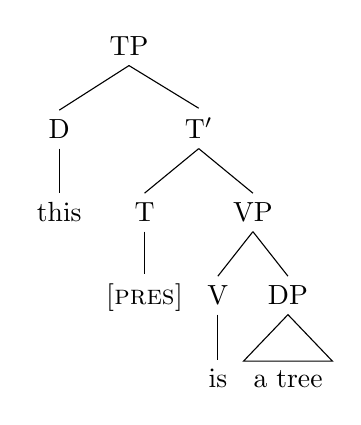
\begin{tikzpicture}
    \Tree [.TP [.D this ] [.T$'$ [.T \textsc{[pres]} ] % 
      [.VP [.V is ] [.DP \edge[roof]; {a tree} ] ] ] ]
  \end{tikzpicture}
	    \end{verbatim}


	  \ex 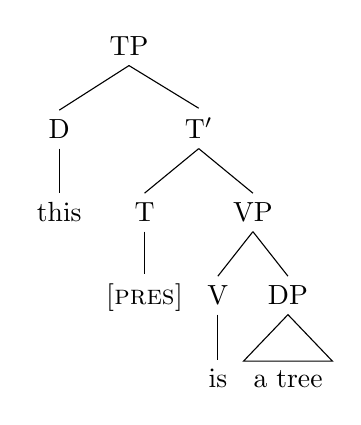
\begin{tikzpicture}
		\Tree [.TP [.D this ] [.T$'$ [.T \textsc{[pres]} ] % 
		  [.VP [.V is ] [.DP \edge[roof]; {a tree} ] ] ] ]
	      \end{tikzpicture}
   
	\end{exe}

      \item Many people swear by TikZ for drawing. One major advantage of TikZ is that it works with any \LaTeX\ compiler, which cannot be said of the older PSTricks package (see below)
      
      \item However, I find the bracket notation too cumbersome for more complicated trees. I also find the syntax for drawing arrows a bit too unintuitive, but that's me.
      
    \end{itemize}
    
  \subsubsection{forest}\label{S:Forest}
  
    \begin{itemize}
      \item Another TikZ-based package that uses bracket notation is \verb|forest|.
      
      \item It uses a slightly different bracket notation than \verb|tikz-qtree|.
      
      \begin{exe}
        \ex\begin{verbatim}
\begin{forest}
  [TP [D [this] ] [T$'$ [T [{\textsc{[pres]}}] ] %
    [VP [V [is] ] [DP [{a tree}, roof] ] ] ] ]
\end{forest}
	    \end{verbatim}
	  \ex\begin{forest}
		  [TP [D [this] ] [T$'$ [T [{\textsc{[pres]}}] ] %
		    [VP [V [is] ] [DP [{a tree}, roof] ] ] ] ]
		\end{forest}

      \end{exe}

    \end{itemize}


  \subsubsection{pst-jtree}
  
    \begin{itemize}
       
      \item The \verb|pst-jtree| package is a PSTricks-based tree-drawing package. Unlike the ones discussed above, it is does not use bracket notation but has it's own syntax.
      
      \item It is not known for being user-friendly, but it is very powerful and, with practice, will let you draw almost any tree.\footnote{It was created with producing multidominant trees in mind.}
            
	\begin{exe}
	  \ex
	    \begin{verbatim}
	\begin{jtree}
	  \! = {TP}
	    <left>[]{D}(<vert>[]{this})             ^<right>[]{T$'$}
	    <left>[]{T}(<vert>[]{\textsc{[pres]}})  ^<right>[]{VP}
	    <left>[]{V}(<vert>[]{is})               ^<right>[]{DP}
	    <vartri>[]{a tree}.
	  \end{jtree}
	    \end{verbatim}

	  \ex
	    \begin{jtree}
	      \! = {TP}
		<left>[]{D}(<vert>[]{this})		^<right>[]{T$'$}
		<left>[]{T}(<vert>[]{\textsc{[pres]}})	^<right>[]{VP}
		<left>[]{V}(<vert>[]{is})		^<right>[]{DP}
		<vartri>[]{a tree}.
	    \end{jtree}

	\end{exe}

	
      \item The big drawback to \verb|pst-jtree| is that it uses PSTricks for drawing, which is incompatible with pdf\LaTeX. You must use (plain) \LaTeX\ to compile documents that use \verb|pst-jtree|.
	
      \item Another issue is that \verb|pst-jtree| sometimes requires the use to make very fine-grained control how a tree appears. Getting the spacing between nodes right can be a pain.
      
	  \begin{itemize}
	  
	    \item Packages like \verb|qtree| automatically adjust the space between nodes, but sometimes this leads to comically big trees.
	  
	  \end{itemize}

    \end{itemize}

      
  \subsection{Fonts and typographical stuff}\label{S:Fonts}
  
%   \subsection{Changing fonts}
  
    \begin{itemize}
      \item The default font in \LaTeX\ is Computer Modern. It is instantly recognizable, but has a reputation for not being pleasant to read.
      
      \item Depending on how you compile your document, your options for what fonts to use can be rather limited.
      
	  \begin{itemize}
	  
	    \item Due to its age, \LaTeX\ wasn't designed with modern fonts in mind. This means that \LaTeX\ cannot, in general, use any font available on your computer. Most fonts that you will use will come as part of your \LaTeX\ distribution.
	    
	    \item However, if you use \XeLaTeX, you can use either \LaTeX\ native fonts or any font installed on your computer.
	  
	  \end{itemize}
	  
	\item I discuss each of these options below.
	
    \end{itemize}
    
  \subsubsection{Font selection under \LaTeX\ and pdf\LaTeX}
    
    \begin{itemize}
      
      \item Most \LaTeX\ distributions make available a large number of alternative fonts. The Danish \TeX\ User Group keeps a pretty good list with many samples and details about each at the \LaTeX\ Font Catalogue: \url{http://www.tug.dk/FontCatalogue/}.
      
      \item For various reasons, many authors must set documents in Times. If so, you should use either the package \verb|mathptmx| or the packages \verb|newtxtext| and \verb|newtxmath| together, as this will ensure that both text and math will be set in Times.\footnote{For various technical reasons that remain obscure to me, \LaTeX\ uses distinct fonts in math mode and regular text. Not all fonts support math mode.}
      
      \item Other popular options include Linux Libertine (using the \verb|libertine| package) and Bitstream Charter (\verb|\usepackage[bitstream-charter]{mathdesign}|)

      \item Many fonts other than Computer Modern (including those listed above) require using the \verb|fontenc| package to ensure the right font encoding is used. If you choose a font from the \LaTeX\ Font Catalogue, it will tell you how to use this package.
      
    \end{itemize}

  \subsubsection{Using \XeLaTeX}
  
    \begin{itemize}
      \item \XeLaTeX\ is a modern implementation of \LaTeX\ that has full \textsc{utf8} support and can use TrueType and OpenType fonts installed on your computer.
      
	  \begin{itemize}
	  
	    \item As discussed in Section \ref{S:Compiling}, you must use the \XeLaTeX compiler at the command line rather than \LaTeX\ or pdf\LaTeX.
	  
	  \end{itemize}
      
      \item The usual way of choosing a font for use with \XeLaTeX\ is with the \verb|fontspec| package, though I recommend using \verb|mathspec| because it will ensure that material in math mode will be set in the same font rather than in Computer Modern.
      
      \item To select fonts with \verb|mathspec|, the following basic commands will get you started:
      
	  \begin{tabular}{ll}
	    \textbf{Command:}	& \textbf{Effect:} \\
	    \verb|\setallmainfonts[<options>]{<font name>}|	& Sets main font and math font.\\
	    \verb|\setsansfont[<options>]{<font name>}|		& Sets sans serif font. \\
	    \verb|\setmonofont[<options>]{<font name>}|		& Sets typewriter font. \\
	  \end{tabular}

	\item So, for example, if you want to set your document in Adobe's Arno Pro, you would use the command \verb|\setallmainfonts{Arno Pro}|.
	
	  \begin{itemize}
	  
	    \item Be careful here, though. The font name has to match exactly what your system thinks the font is called. You may need to check your system's font settings to be sure.  
	  
	  \end{itemize}
	  
    \end{itemize}

    
  \subsection{Non-English languages and scripts}
  
    \begin{itemize}
      \item Owing to its age, \LaTeX's support for non-Latin scripts is not particularly good. 
      
	\begin{itemize}
	
	  \item \LaTeX\ was first released in 1983. Unicode would not come into existence until the late 80s.
	  
	  \item Additionally, most modern font formats (like TrueType and OpenType) had not been invented yet.
	  
	    \begin{itemize}
	    
		\item This means that standard (pdf)\LaTeX\ does not let you use any font on your computer. In general, you must use fonts set for use with \LaTeX. See Section \ref{S:Fonts}.
		
% 		\item However, if you use \XeLaTeX, you can use any font/typeface on your computer.
	    
	    \end{itemize}
	  
	  \item For various technical reasons, there are different econdings for typefaces. If you want to use a font other than the default \
	
	\end{itemize}
      
      \item If you want to diacritics or accent marks on Latin characters, there is fairly good native support for this if you are willing to use \LaTeX's built-in commands.
      
      \item If you want to type in characters directly, you must use the package \verb|inpuntenc|, with the \verb|utf8| option:
      
	\begin{verbatim}
	  \usepackage[utf8]{inputenc}
	\end{verbatim}

	If you don't do this, nothing will appear if you type a character like \texttt{\"{o}} .
	
      \item If you want to change various section headings, dates, hyphenation rules, and other language-specific parts of the document, use the \verb|babel| package:
      
	\begin{verbatim}
	  \usepackage[<language>]{babel}
	\end{verbatim}

      \item However, if you want/need to use non-Latin characters, you should really consider using \XeLaTeX! \XeLaTeX\ supports modern \textsc{utf8} encoding natively and works with your system fonts.
    \end{itemize}
    
  \subsection{Phonetic symbols}
  
    \begin{itemize}
      \item If you need to use \textsc{ipa} symbols in your document, the \verb|tipa| package is absolutely excellent.
      
      \item \verb|tipa| provides many shortcut codes for typing \textsc{ipa} symbols quickly. For instance, the code \verb|\textipa{[f@"nE.RIks]}| produces the following output: \textipa{[f@"nE.RIks]}

	\item The \verb|tipa| package is not compatible with \XeLaTeX. If you want to use \verb|tipa| codes with the \verb|\textipa| command, use the \verb|xunicode| package, which re-implements its functionality in \XeLaTeX.
	
	  \begin{itemize}
	  
	    
	    \item To do this, you must use a font that includes \textsc{ipa} symbols. If your main font does not include these, you can specify an \textsc{ipa}-specific font using the following commands (assuming you are using \verb|xunicode| and \verb|fontspec|):
	    
		\begin{verbatim}
\newfontfamily{\mytipa}[Scale=MatchLowercase]{<IPA Font Name>}
\renewcommand\useTIPAfont{\mytipa}%

		\end{verbatim}

	  
	  \end{itemize}
    \end{itemize}

  \subsection{Tableaux}
  
    \begin{itemize}
      \item It is possible to press \verb|tabular| environments into service here, but it can be hard to do fancy (and important) stuff like draw dashed lines between unranked constraints.
      
	\begin{tabular}{|lll||c@{\ :\ }c|c|}
	  \hline
	    & & \textipa{/patak/} 	& \textsc{NoCoda}	& \textsc{Max}	& \textsc{Dep} \\
	  \hline\hline
	    a. & $\rightarrow$ & \textipa{pataka} & 		& 		& *	\\
	  \hline
	    b. & & \textipa{pata} 	& 			& *		& 	\\
	  \hline
	    c. & & \textipa{patak}	& *			& 		& 	\\
	  \hline
	\end{tabular}

      
      \item However, if you want professional looking tableaux, Nathan Sanders' \verb|OTtablx| package creates excellent looking tableaux. You can even make complicated comparative tableaux:
      
	\begin{OTcomparative}{3}
	  \OTsolids{2}
	  \OTdashes{1}
	  \OTtoprow[\textipa{/patak/}]{\textsc{NoCoda}, \textsc{Max}, \textsc{Dep}}
	  \OTcandrow[\OThand]{pataka}{ 0, 0, 1}
	  \OTcandrow[]{pata}{ 0, \OTcompviol[W]{1}, \OTcompviol[L]{0}}
	  \OTcandrow[]{patak}{\OTcompviol[W]{1}, 0,\OTcompviol[L]{0} }
	\end{OTcomparative}

      \item As with jTree, mentioned above, \verb|OTtablx| uses PSTricks, and so it cannot be used with pdf\LaTeX.
	
    \end{itemize}
    
  \subsection{Autosegmental diagrams}\label{S:Autoseg}
  
    \begin{itemize}
  
	\item The only package I know of specifically designed for drawing autosegmental diagrams is \verb|pst-asr|, which uses PSTricks, though I'm sure there must be a TikZ package for drawing autosegmental diagrams as well. 
	
	\item The code for \verb|pst-asr| is complicated, and the learning curve is notoriously steep, but it makes great diagrams.
  
    	  \begin{exe}
    	  
	    \ex
\begin{verbatim}
\newtier{foot}    
\newtier{word}    
\tiershortcuts
  \asr[reptype=nots,foot=(sy) 4.5ex (Ft), word=(sy) 10ex (Wd), xgap=1.25em]
  \2m{\textipa{\ae}}\2f{\textipa{2}}\3k{\textipa{I}}{\textipa{N}}
  \2n{\textipa{I}}\2t{\textipa{o}}\2b{\textipa{@}}|
  \@(5.75,foot){Ft}\-(2.5,sy)\-(5,sy)
  \@(1.5,foot){Ft}\-(0.5,sy)\-[border=1pt](7.5,sy)
  \@(10.5,foot){Ft}\-(9.5,sy)\-(11.5,sy)
  \@(5.75,word){Wd}\-(1.5,foot)\-(5.75,foot)\-(10.5,foot)
\endasr

\end{verbatim}
	    
	    
	  \ex[*]{Ma-fucking-nitoba}\smallskip
	    \newtier{foot}    
	    \newtier{word}    
	    \tiershortcuts
	    \asr[reptype=nots,foot=(sy) 4.5ex (Ft), word=(sy) 10ex (Wd), xgap=1.25em]
		\2m{\textipa{\ae}}\2f{\textipa{2}}\3k{\textipa{I}}{\textipa{N}}\2n{\textipa{I}}\2t{\textipa{o}}\2b{\textipa{@}} 
		|
		\@(5.75,foot){Ft}\-(2.5,sy)\-(5,sy)
		\@(1.5,foot){Ft}\-(0.5,sy)\-[border=1pt](7.5,sy)
		\@(10.5,foot){Ft}\-(9.5,sy)\-(11.5,sy)
		\@(5.75,word){Wd}\-(1.5,foot)\-(5.75,foot)\-(10.5,foot)
	    \endasr
			
	  \end{exe}
	  
	  \item As with \verb|OTtablx| and \verb|pst-jtree|, this package uses PSTricks and so cannot be compiled with pdf\LaTeX.
	  
% 	    \begin{itemize}
% 	    
% 		\item If used with 
% 	    
% 	    \end{itemize}
	  

    \item The \verb|forest| package discussed in Section \ref{S:Forest} can also draw autosegmental tree diagrams. The following is taken from the \verb+forest+ documentation:
    
	\begin{exe}
	  \ex
	    \begin{verbatim}
\begin{forest} GP1 [
  [O[x[f]][x[r]]]
  [R[N[x[o]]][x[s]]]
  [O[x[t]]]
  [R[N[x]]]
]\end{forest}
	    \end{verbatim}
	    
	  \ex
	    \begin{forest} GP1 [
		[O[x[f]][x[r]]]
		[R[N[x[o]]][x[s]]]
		[O[x[t]]]
		[R[N[x]]]
	    ]\end{forest}

	\end{exe}

	\end{itemize}

  \subsection{Semantic formulas}
  
    \begin{itemize}
      \item \LaTeX's native mathmode provides a lot of functionality for typesetting semantic formulas and denotations. A few extra packages are occasionally necessary for 
      
      \item The package \verb|stmaryrd| provides standard denotation brackets $\llbracket.\rrbracket$
      
      \item The packages \verb|amssymb| and \verb|amsmath| also provide additional functionality
      
    \end{itemize}
    
    \begin{exe}
    \ex\begin{verbatim}
	  $\llbracket\mbox{the}\rrbracket = \lambda P. \lambda Q. \exists x. %
      [Q(x) \wedge \forall y. [P(y) \rightarrow x = y]]$
       \end{verbatim}

    \ex[]{$\llbracket\mbox{the}\rrbracket = \lambda P. \lambda Q. \exists x. %
      [Q(x) \wedge \forall y. [P(y) \rightarrow x = y]]$}
    \end{exe}


  
%   \subsubsection{What if I don't want to use \XeLaTeX?}
%     
%     \begin{itemize}
% 	
%       \item Some scripts, like Cyrillic have fairly good support through the \verb|T2| encoding. You can load this with the \verb|fontenc| package:
%       
% 	\begin{verbatim}
% 	  \usepackage[T2]{fontenc}
% 	\end{verbatim}
% 
%       \item Even then, if you want to use non-Latin characters, things become even more difficult.
%       
% 	\begin{itemize}
% 	
% 	  \item Chinese, Japanese, and Korean have historically been supported in \LaTeX\ through the \verb|CJK| package. Getting this to work is not known to be easy.\footnote{A lot of this boils down to getting and installing the right sorts of fonts. It is doable, but not very straightforward.}
% 	  
% 	  \item Arabic script and Hebrew are also supported
% 
% 	
% 	\end{itemize}
%       
%       \item 
% 	
%     \end{itemize}
    
  \subsection{Graphics and images}
  
    \begin{itemize}
      \item Another place that \LaTeX\ shows its age is in how it handles graphics,\footnote{The \textsc{pdf} standard dates to 1993; \textsc{jpeg}, to 1992; and \textsc{gif}, to 1987. \LaTeX\ was first released in 1983 and was not created with these modern image formats in mind.} and this is probably one of the places it is most frustrating to use.
      
      \item \LaTeX\ has no native support for graphics. Graphics and images must be imported with the \verb|graphicx| package.
      
      \item The frustrating thing is that the graphics formats you can use in a document are different depending on which method you use to compile your document.
      
	\begin{itemize}
	
	  \item latex $\rightarrow$ dvips $\rightarrow$ ps2pdf \\	  
	    You can import postscript graphics (.eps files), and nothing else. If you want to use graphics with this mode, you must convert them to .eps files first.
	    
	  \item pdflatex \\
	    You can import jpeg, pdf, and png files, amongst others. It can also use .eps file (but secretly converts them to .pdf format).
	    
	  \item xelatex \\
	    \XeLaTeX\ supports most graphics formats. 
	
	\end{itemize}
      
      \item The reason this leads to frustration is that you might need to use a specific compiler for other reasons. For instance, if you use \verb|pstricks| for drawing trees, you won't be able to use pdf\LaTeX.%\footnote{\XeLaTeX\ allows one to use \verb|pstricks| as well as several graphics formats.}
	
	
      \item If you need to import and manipulate .pdf documents, the \verb|pdfpages| is extremely useful.
    \end{itemize}

  \subsection{Drawing}

    \begin{itemize}
    
      \item I use the \verb|pst-node| package from PSTricks for drawing arrows between things.
      
	\begin{exe}
	  \ex[*]{\rnode{wh}{Who$_i$} did Bill meet Sally [$_{Adjunct}$ before he talked to \rnode{trace}{$t_i$}]?}
	    \ncbar[angle=-90, linearc=0.25ex, linestyle=dashed, nodesep=2pt]{->}{trace}{wh}\ncput*{*}
	\end{exe}
	
      \item As mentioned above, you can also use \verb|tikz| to draw.

    \end{itemize}

  
  \section{Bibliography management and citations}\label{S:Bib}
  
    \begin{itemize}
      \item \LaTeX\ has some native capacity for in-text citations, but this functionality is usually extended with various packages.
      
	  \begin{itemize}
      
	    \item Probably the most common package for bibliography and references is \verb|natbib|, which interfaces with Bib\TeX.
	    
	    \item More recently, the \verb|biblatex| package has been developed, interacting with the biber system. This system is more powerful and flexible than \verb|natbib|.
      
	  \end{itemize}
	  
	\item Each of these systems is fairly different under the hood, but most of the user-end functionality is essentially the same.
	
	  \begin{itemize}
	  
	    \item Users create a bibliography file, which is a database that contains information about references the author will use in a document.
	    
	    \item Various citation commands provided by \verb|natbib|/\verb|biblatex| are responsible for citing the appropriate references in the bibliography.
	    
	    \item When the document is compiled, \LaTeX\ finds the references in the bibliography file that match those cited in the document.
	    
	    \item Compiling the document adds the cited references to the references section and adds in-line citations to the document.
	  
	  \end{itemize}
	  
    \end{itemize}
    
  \subsection{The bibliography file}
  
  \subsection{Citing references}
  
  \subsection{Formatting references and citations}

  \section{Slides and posters with Beamer}
  
    \begin{itemize}
      \item You can use \LaTeX\ to create presentation slides and posters using the Beamer document class.\footnote{The name \emph{beamer} comes from the German loanword for a projector.}
      
%       \item 
    \end{itemize}

  \subsection{Presentations with Beamer}
  
    \begin{itemize}
      \item Beamer is designed to create presentation slides (\emph{frames} in its terms).
      
      \item Beamer includes special commands for creating and laying out slides, controlling the flow of information.
      
      \item Each slide is defined in a frame environment, which contains standard \LaTeX\ code:
      
	\begin{verbatim}
	  \begin{frame}{This is the title of the slide}
	    The following list will appear after a pause:\pause
	      \begin{itemize}
	        \item This is the first item.
	        \item This is the second item.
	      \end{itemize}
	  \end{frame}
	\end{verbatim}

      \item The output is .pdf file that can be viewed in any .pdf viewer.
	
    \end{itemize}

  
  \subsection{Make a real handout with the \texttt{beamerhandout} package}
  
    \begin{itemize}
      \item Printing out your slides 6-up is for PowerPoint users. The \verb|beamerhandout| package makes it easy to convert your slides into a true handout!
    \end{itemize}

  \subsection{Posters using \texttt{beamerposter}}
  
    \begin{itemize}
      \item The \verb|beamerposter| package makes one huge Beamer frame to be used as a poster.
    \end{itemize}

  
  \section{Additional resources}
  
    \begin{itemize}
      \item The \LaTeX\ Wikibook is a good, free resource: \url{https://en.wikibooks.org/wiki/LaTeX/}
      
	\begin{itemize}
	
	  \item The chapter on Linguistics has more examples and some different package examples.
	
	\end{itemize}
      
      \item The ShareLaTeX documentation at \url{https://www.sharelatex.com/learn/Main_Page} is very comprehensive! 
      
      \item When things fail, check out StackExchange!
    \end{itemize}


\end{document}
